Figure \ref{fig:final-bent-part} shows the final bent sheet metal part that is sent to the project partner for assessment and measurement. The test part is scanned in a 3D scanner for measurement of all bending angles and surface structure. There are no discrepancies found in any of the test parts bent by the KR1410 robotic workcell. This shows that the inspection camera is working correctly and the angle difference between two parts is only due to surface imperfections. Hence, a bigger tolerance in the inspection camera angle measurement still gives correctly bent part.

\begin{figure}[h]
    \centering
    \begin{subfigure}{0.48\textwidth}
        \centering
        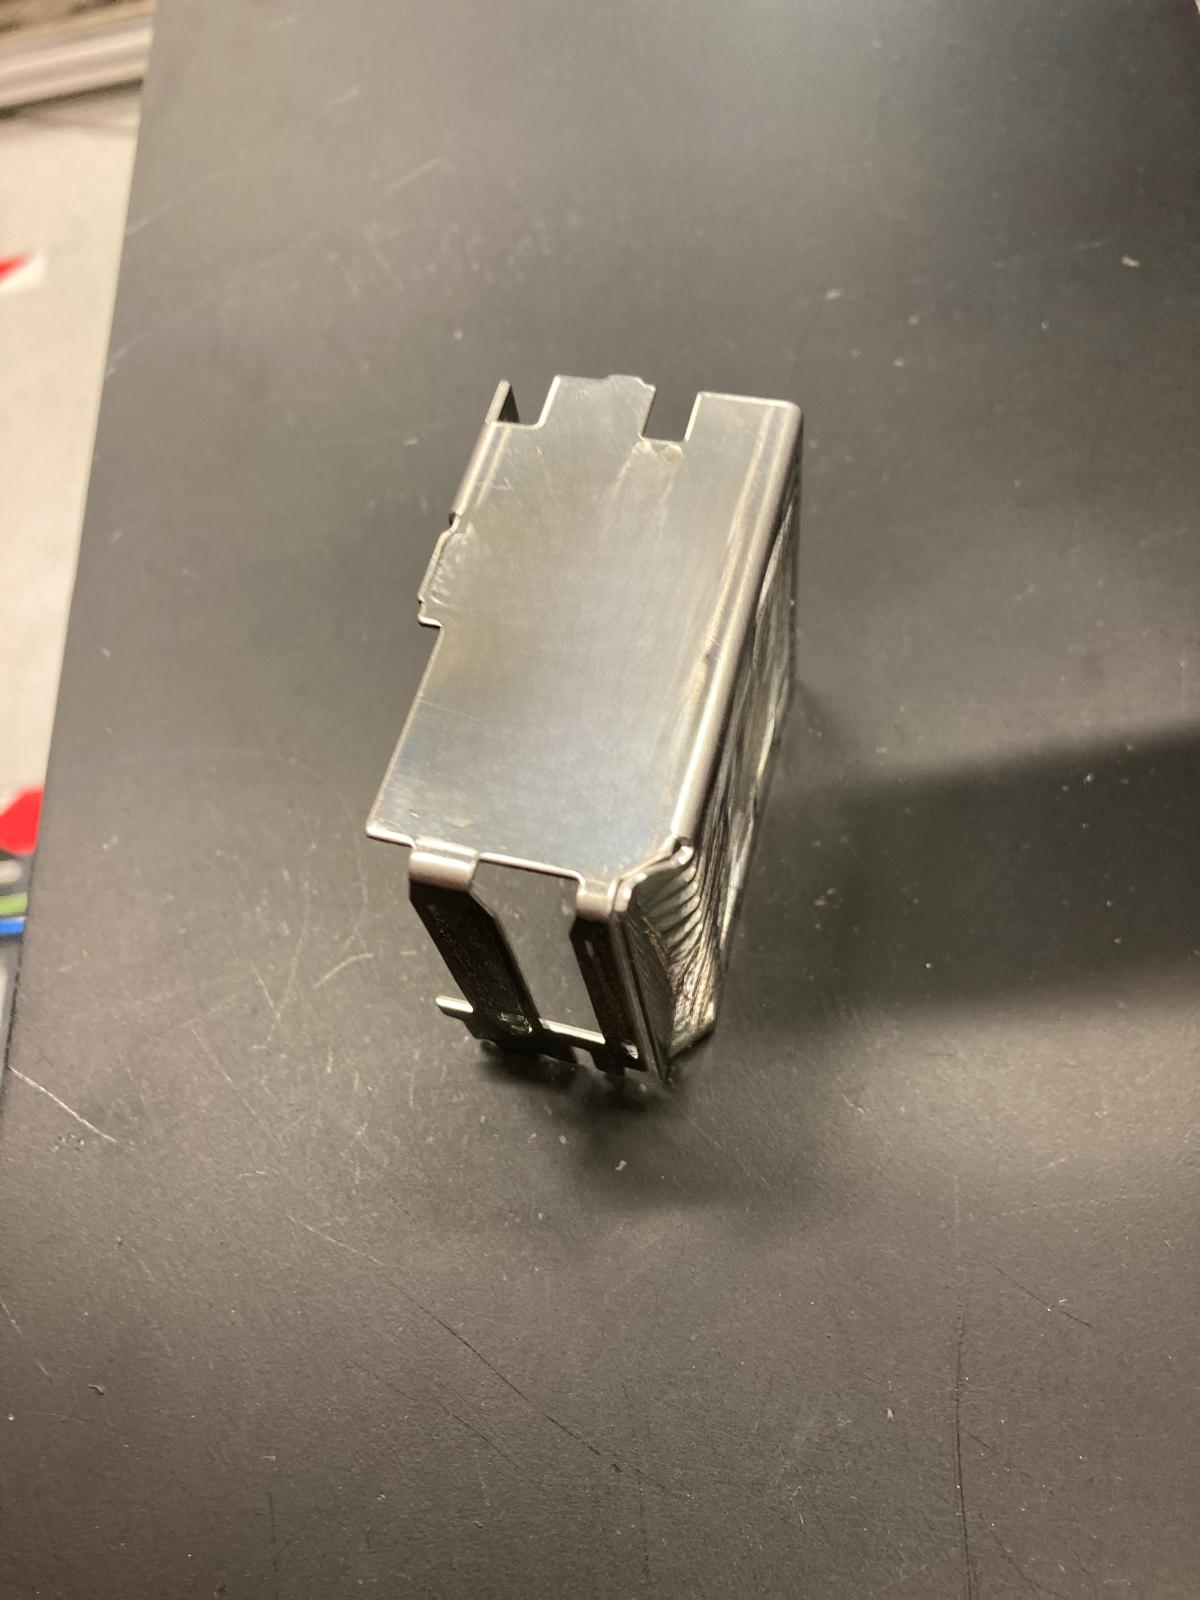
\includegraphics[width=\textwidth]{figures/bending/final-part02.png}
        \caption{}
        \label{subfig:final-part1}
        \vspace{0.5cm}
    \end{subfigure}\hspace{0.25cm}
    \begin{subfigure}{0.48\textwidth}
        \centering
        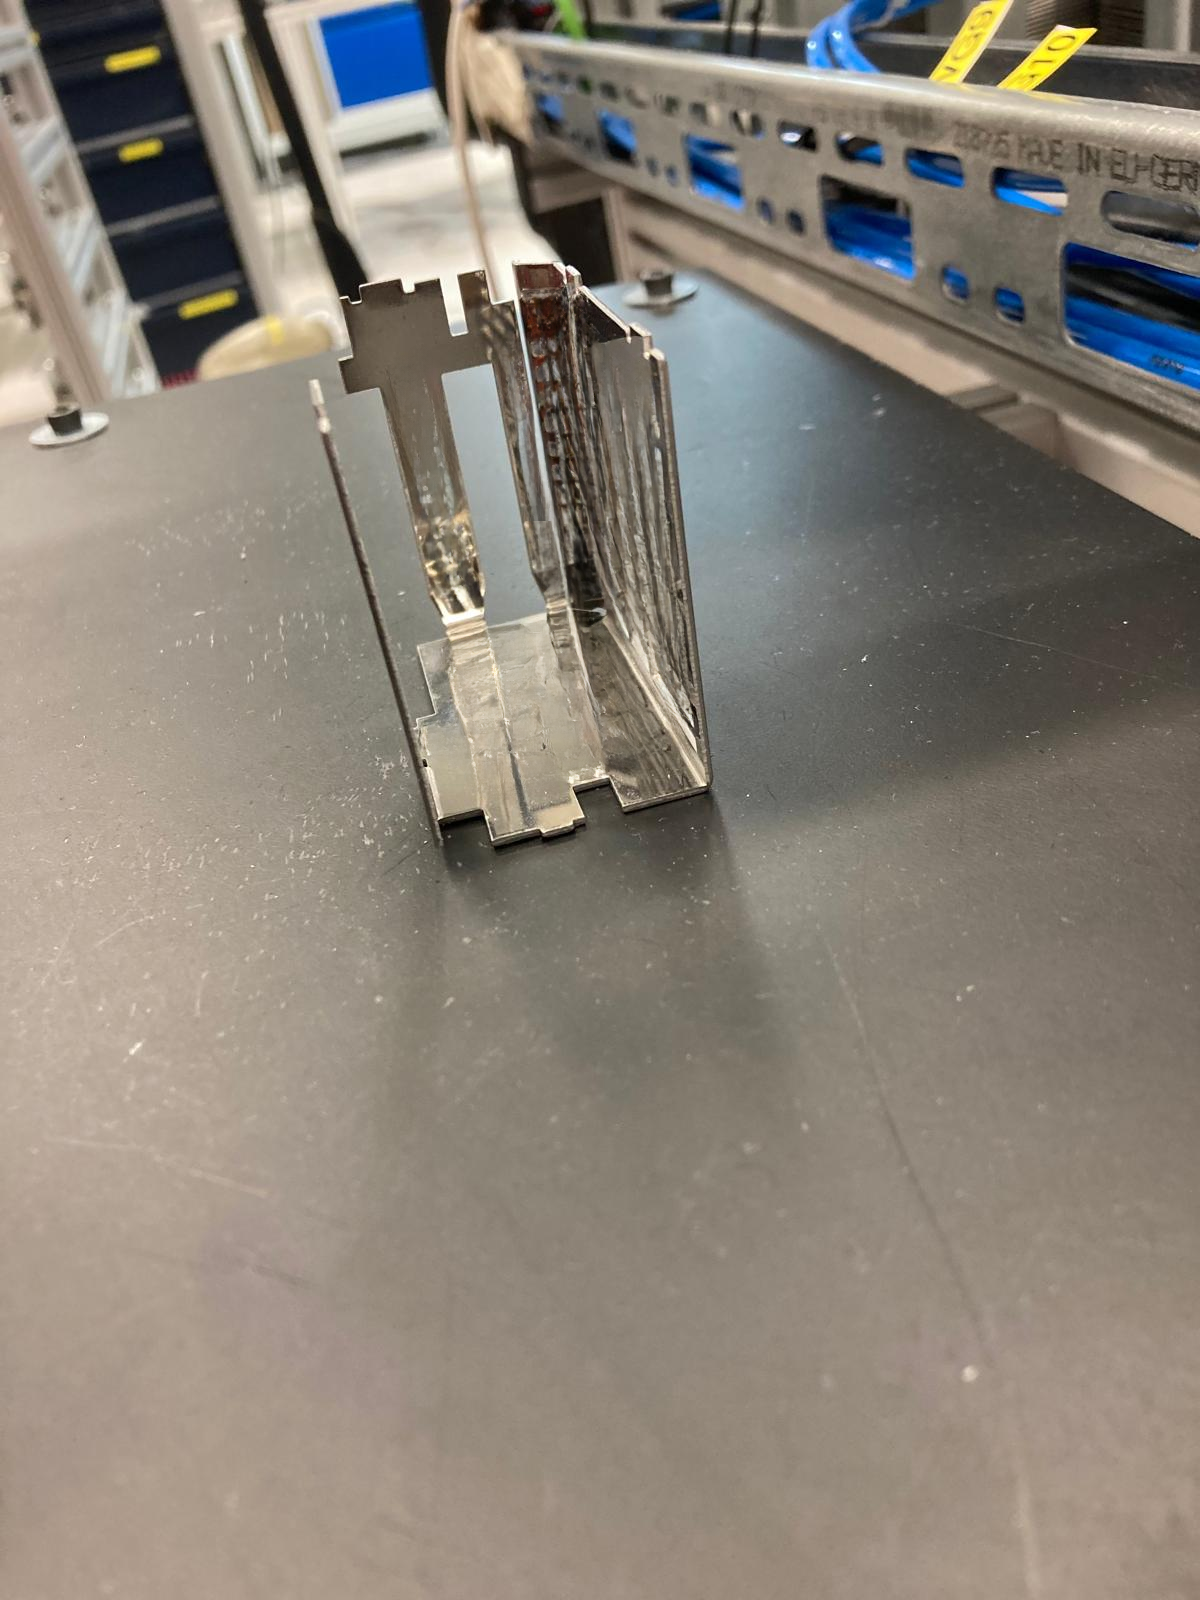
\includegraphics[width=\textwidth]{figures/bending/final-part01.png}
        \caption{}
        \label{subfig:final-part2}
        \vspace{0.5cm}
    \end{subfigure}\hspace{0.25cm}

    \caption{Final bent sheet metal part (a) top view (b) bottom view}
    \label{fig:final-bent-part}
\end{figure}